\documentclass[platex,a4j,10pt,twoside,twocolumn,dvipdfmx]{jsarticle}
\usepackage[ipaex]{pxchfon} % overleaf用
%

\setlength{\textheight}{240mm}

\setlength{\textwidth}{170mm}
\setlength{\oddsidemargin}{-15mm}
\setlength{\evensidemargin}{-15mm}
\addtolength{\textwidth}{15mm}

\setlength{\textwidth}{\paperwidth}
\setlength{\oddsidemargin}{-5.4truemm}  % 左の余白を20mm(=1inch-5.4mm)に
\setlength{\evensidemargin}{-5.4truemm} % 
\addtolength{\textwidth}{-40truemm}     % 右の余白も20mmに

\setlength{\topmargin}{-15mm}
\setlength\textfloatsep{3mm}
\setlength\floatsep{2mm}

\columnsep 1.0cm
%\setlength\abovecaptionskip{-3mm} %キャプションの前に挿入されるスペース

%------------------------------------------------------------



%------------------------------------------------------------
\usepackage[dvipdfmx]{graphicx}
% \usepackage{graphicx}
\usepackage{dendentitle}
\usepackage{mediabb}
\usepackage{url}
%\usepackage[dvipdfmx]{color}
\usepackage{color}
\usepackage{amsmath,amssymb,amsopn,bm}
\usepackage{subfig}
\usepackage{multirow}
\usepackage{cite}
\usepackage{comment}
%\usepackage{natbib}
\usepackage[table,xcdraw]{xcolor}

%------------------------------------------------------------ 関数定義
\renewcommand{\baselinestretch}{0.95}
\renewcommand{\figurename}{Fig.~}
\renewcommand{\tablename}{Table~}
\graphicspath{{./images/}}
\newcommand{\Tref}[1]{Table~\ref{#1}}
\newcommand{\Eref}[1]{式(\ref{#1})}
\newcommand{\Fref}[1]{Fig.~\ref{#1}}
\newcommand{\Sref}[1]{第\ref{#1}章}
\newcommand{\SSref}[1]{第\ref{#1}節}
\newcommand{\argmin}{\mathop{\rm arg~min}\limits}
\newcommand{\argmax}{\mathop{\rm arg~max}\limits}
\newcommand{\etal}[0]{\emph{et al}.~}

%タイトル
\title{eBPFを用いたセキュリティシステムに関する調査 \\
\large{\textgt{A Survey on Security Systems with eBPF}}}
\author{電子情報学専攻 修士課程1年 48-236427 手塚 尚哉}
\date{2023年11月21日}

\begin{document}
\makedendentitle{電子情報学輪講資料}{宮本研究室}

% TODO: Update the abstract with the final content. Note that this abstract is a placeholder 
% and should be updated with the final content.

\section*{Abstract}
In the complex arena of cybersecurity, evasive malware,
such as shadow attacks that obscure malicious activities
through multiple processes, challenge conventional detection methods.
This paper introduces an innovative detection and analysis methodology
using Extended Berkeley Packet Filter (eBPF) technology to counteract these threats.
eBPF facilitates real-time, in-depth monitoring of system operations,
enabling the identification of sophisticated malware behaviors.

We leverage eBPF to trace process interactions and system calls,
identifying malicious patterns indicative of shadow attacks.
This approach distinguishes between legitimate and malicious activities
by analyzing process executions and network communications.
Despite challenges like data volume and behavior differentiation,
we apply smart filtering and machine learning to enhance detection accuracy.

Our research showcases eBPF's potential in detecting complex malware
through case studies, emphasizing the need for advanced analysis techniques
in cybersecurity.
This work contributes significantly to understanding and mitigating advanced malware threats,
proving eBPF as a vital tool in modern cybersecurity defenses.


\section{はじめに}
backgroundのまとめ \& 本稿の構成

\section{eBPF}
  \subsection{Berkeley Packet Filter}
    StevenとVan \cite{mccanne1993bsd}は1993年に,Unix系のOS上でパケットキャプチャを効率的に行うためのアーキテクチャである
    BSD Packet Filterを提案した.以下,Berkeley Packet Filterを「BPF」と表記する. \\
    論文発表当時のパケットキャプチャでは,カーネル空間で取得したパケットをすべてユーザー空間にコピーしてからフィルタリングしていて,
    これが無駄なオーバーヘッドの原因となっていた.
    \cite{mccanne1993bsd}は特殊な32ビット命令で記述されたプログラムを解釈して
    フィルタリングを行う疑似マシン (BPF pseudo-machine) を考案し,それをカーネル空間で動作させることでこの問題に対処した.
    既存のシステムとの比較では,BPFは最大で20倍程度高速に動作した.
    BPFのアーキテクチャの概要を\Fref{img:bpf_old}に示す.
    
    BPFはLinuxカーネルのv2.1.75にてLinux Socket Filterという名前で導入され,\texttt{tcpdump}コマンドの高速化のために使われた.
    
  \subsection{BPFの拡張}
    BPFはLinuxカーネルのv3.18にて大幅に改修,拡張が行われ,extended BPFすなわちeBPFと呼ばれるようになった \cite{Linux31836:online}.
    拡張された部分は多岐にわたるが,代表的なものを以下に列挙する \cite{learning-ebpf}.
    \begin{itemize}
      \item BPF命令セットが32ビットから64ビットに書き直され,実行効率が向上した.
      \item eBPF mapが導入され,ユーザー空間とカーネル空間の間でデータを共有する手段が追加された.
      \item eBPFプログラムが安全に実行できることを検証するeBPF verifierが追加された.
    \end{itemize}
    \begin{figure}[tp]
      \begin{center}
        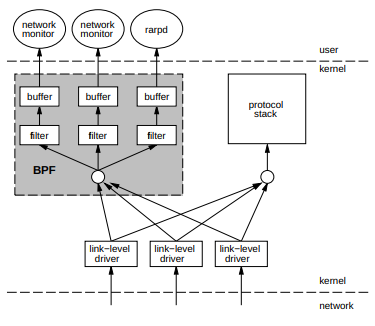
\includegraphics[width=\columnwidth]{./img/bpf_overview.png}
      \end{center}
      \caption{The overview of BPF architecture. It accelerates packet capture
                by performing filtering in the kernel space. \cite{mccanne1993bsd}}
      \label{img:bpf_old}
    \end{figure}
    
    また,eBPFがカバーする領域も拡大していった.ネットワークの文脈では,Linuxのネットワークスタックの様々なレイヤー,例えばUnix socket
    やネットワークデバイスなどを扱えるようになった.加えてeBPFプログラムはLinuxシステムのパフォーマンストレーシングやセキュリティ向上にも
    利用できるようになり,"BPF"という単語は本来の意味である"Berkeley Packet Filter"を失い独立した単語として使われるようになっていった.
    
    便宜上,v3.18における拡張以前のBPFをclassical BPF,あるいはcBPFと呼ぶことがある.
  
  \subsection{eBPFのアーキテクチャ}
    eBPFのアーキテクチャの概要を\Fref{img:ebpf-system}に示す.以下,\Fref{img:ebpf-system}を参照しながら重要な
    処理フローについて説明する.
    \begin{figure}[tp]
      \begin{center}
        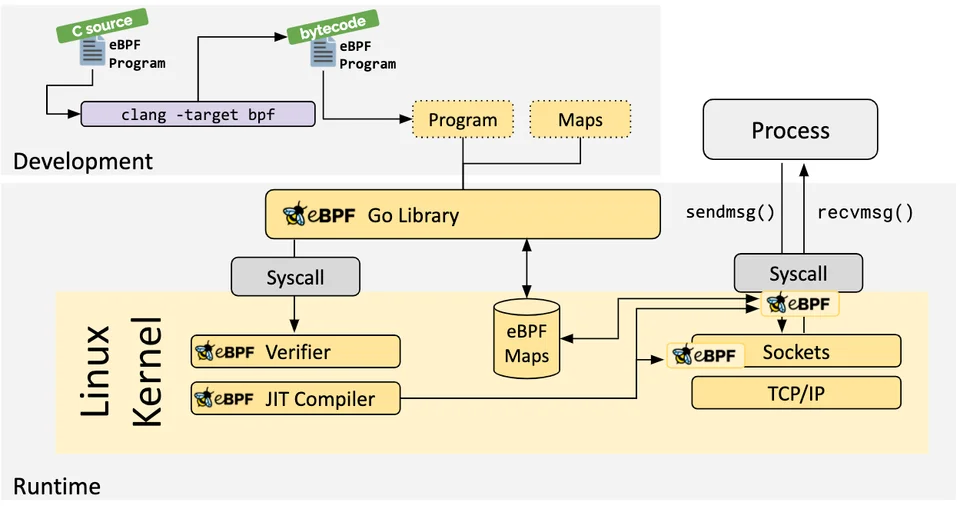
\includegraphics[width=\columnwidth]{./img/ebpf_system.png}
      \end{center}
      \caption{The overview of eBPF architecture. This figure shows how eBPF programs are compiled, verified, and executed.
      \cite{WhatiseB29:online}}
      \label{img:ebpf-system}
    \end{figure}

    \subsubsection{Event-Driven Architecture}
    eBPFはevent-drivenである.カーネル内でのイベントにeBPFプログラムをフックし,
    イベントが発生したら所定の処理を行う,という仕組みである.
    eBPFプログラムは動的にロードまたは削除することが可能である.
    
    eBPFがフックできるイベントはカーネルのソースコード \footnote{\texttt{include/uapi/linux/bpf.h}} においてProgram Typeとして定義されている.
    Program Typeをイベントの種別ごとに分類すると,以下のようなものが挙げられる.
    \begin{itemize}
      \item XDP: ネットワークデバイスにパケットが到着したとき,カーネル空間にデータがコピーされる前にパケットを操作するためのイベント.
      \item tracing: カーネル関数の呼び出しやトレースポイントの通過を検知するためのイベント.
      \item LSM: Linux Security Moduleを利用してセキュリティポリシーを適用するためのイベント.
    \end{itemize}
    
    このようなイベントが発生したとき,eBPFプログラムはProgram Typeに応じた処理を実行する.
    例えばXDPのイベントにフックされているプログラムがパケットをacceptするかdropするかを判断する,といった
    処理が可能である.
    
    \subsubsection{eBPF Verifier}
    eBPF verifierはバイトコードに変換されたeBPFプログラムを入力とし,そのプログラムがカーネル上で安全に
    実行できることを検証するプログラムである.バイトコードは\texttt{bpf()}システムコールで
    カーネル上にロードされる (\Fref{img:ebpf-system}の"Syscall") が,verifierによる検証を
    通過しない限りプログラムは実行されない.
    具体的には,メモリアクセス違反を起こさないことやプログラムが正常に終了すること,
    不必要なprivilegeがプログラムに与えられていないことなどが確認されている.
    
    このように,eBPF verifierはeBPFプログラムに制約を課すことで安全性を高めている.
    verifierがeBPFにおいて重要な意味を持つことから,verifierのロジックを数学的に検証する
    研究 \cite{vishwanathan2023verifying}も行われている.
    
    \subsubsection{JITコンパイル}
    verifierを通過したeBPFバイトコードはJITコンパイラによってターゲットのCPU上で直接動作する機械語に変換される.
    これにより実行速度が最適化され,ソースコードから直接コンパイルされたカーネルおよびカーネルモジュールと同程度効率的に
    動作する.

    
\section{関連分野}
  \subsection{カーネルモジュール}
  カーネルモジュールはLinuxカーネル実行時にオブジェクトファイルをロードすることで,
  カーネルのソースコードを変更せずにカーネルの機能を拡張する仕組みの1つである.
  カーネルモジュールには eBPF verifierのような制約がないため,プログラムの自由度は高い.
  しかしカーネルモジュールはカーネルと同じprivilegeで実行されるので,
  脆弱性を埋め込まないように注意して開発を行う必要がある \cite{chen2011linux}.

  Mayerら \cite{mayer2021performance}が指摘するように,カーネルモジュールの作成を避けることができるのはeBPFの長所であると言える.
  
  \subsection{Linux Security Modules}
  LSM (Linux Security Modules) はLinuxカーネルのセキュリティポリシーを実装するためのフレームワークである.
  LSMはアクセス制御に関するカーネル内の処理にフックポイントを提供し,そのポイントにセキュリティポリシーの
  具体的な実装であるセキュリティモジュールを組み込むことができる
  \footnote{セキュリティモジュールはカーネルモジュールのように動的にロードまたはアンロードすることができず,カーネルのビルド時に静的にリンクする必要がある.}.
  カーネルがフックポイントを通過すると,セキュリティモジュールへのコールバックが発行されて強制的にアクセス制御が行われる.
  LSMの処理フローの概要を\Fref{img:lsm-process}に示す.
  \begin{figure}[tp]
    \begin{center}
      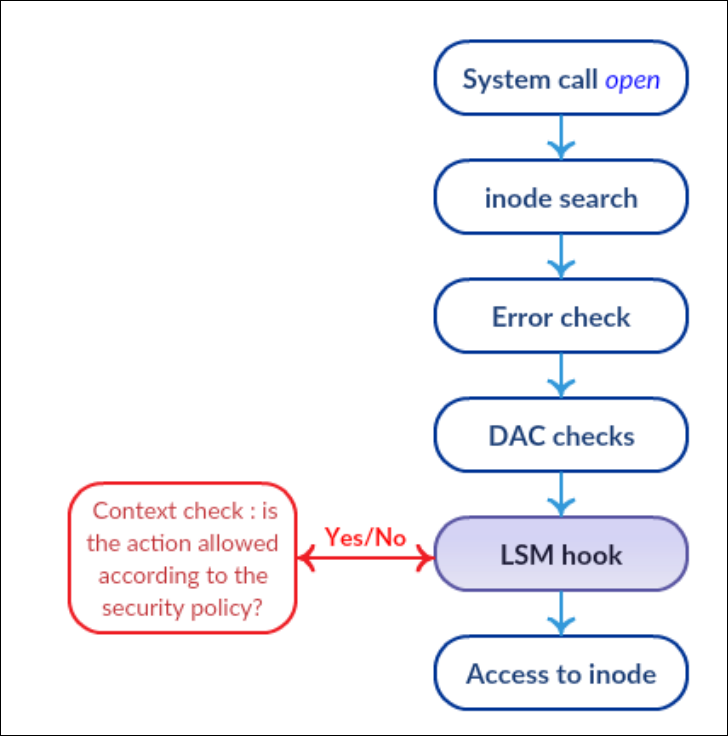
\includegraphics[width=\columnwidth]{./img/lsm-stack-hooks.png}
    \end{center}
    \caption{The process flow of LSM when \texttt{open()} system call is issued. \cite{LinuxSec12:online}}
    \label{img:lsm-process}
  \end{figure}
  LSMはLinuxのcapabilityやSELinuxで利用されている \cite{LinuxSec95:online}.
  
  カーネルv5.17からLSM BPFという機能が追加され,eBPFプログラムをLSMが提供するAPIにフックすることができるようになった.
  
  \subsection{Seccomp}
    SeccompはLinuxで採用されているセキュリティシステムの1つで,あるプロセスが発行することができる
    システムコールを制限する.
    v6.6時点でSeccompの実装はcBPF (eBPFではない) に依存しており,cBPFを用いて
    システムコールのフィルターをプロセスごとに変更することができる.
    この機能をseccomp-bpfと呼ぶ.
    
    SeccompはDocker \cite{Seccomps57:online} やKubernetes\cite{Configur55:online} などの仮想化技術で広く用いられている.
  
  \subsection{クラウドネイティブ}
    クラウドネイティブとは,クラウド基盤を前提としてアプリケーションやシステムを構築および管理するアプローチのことである.
    物理インフラの調達とメンテナンスのコストが不要になるほか,アプリケーションの開発やデプロイが効率的になる点,
    高い可用性が確保できる点がメリットとして挙げられる.
    
    eBPFはクラウドネイティブ環境で幅広く使われている技術で,代表的なプロダクトとしてCilium \cite{CiliumCl38:online}がある.
    Ciliumによってコンテナ間のL3通信を制御したり,セキュリティ機能や可観測性をコンテナ間パケットに付与したりすることができる.
    
    eBPFは以下のような理由でクラウドネイティブ技術とよく適合する.
    \begin{itemize}
      \item ネットワークやシステムコール,アプリケーションのイベントをリアルタイムで監視することができる.
      \item カーネル空間で実行されるためオーバーヘッドが小さく,スケーラビリティを損ねない.
      \item 動的なロードまたはアンロードが可能で,システムの継続的インテグレーション/デリバリーを容易にする.
    \end{itemize} 

\section{既存研究の取り組み}
  これまでに述べたように,eBPFの応用範囲はパケットキャプチャにとどまらず
  ネットワークスタック全般やシステムの監視にまで広がっている.
  本章では,eBPFを活用したセキュリティシステムの中でも,ネットワーク領域の
  事例とそれ以外の領域,そして両方に跨る事例をそれぞれ紹介する.
  
  \subsection{DNSクエリのプライバシーの向上 \cite{rivera2020leveraging}}
  この研究では,DNSクエリのプライバシーを毀損する攻撃についてまとめつつ,それらを緩和する方法の実現が
  既存のシステムでは難しいことを主張している.そしてeBPFを利用して攻撃への対策を効率的に実施する手法を提案している.
  
  \subsubsection{問題}
  DoT (DNS over TLS)やDoH (DNS over HTTPS)といった暗号化プロトコルは,DNSクエリを暗号化することでネットワーク上の攻撃者が
  クエリを盗聴することを防いでいる.しかしDoTやDoHで暗号化されるのはクライアントとキャッシュサーバの間の通信のみであり,
  キャッシュサーバ上でクエリは復号化される.
  したがってキャッシュサーバの運営者,典型的にはISP,はユーザとクエリ情報を結びつけることができるため,
  クエリ情報からユーザのプロファイルを作成するde-anonymizationを試みる危険性がある.
  
  RFC 7626はde-anonymizationへの対策の1つとして,アプリケーションごとにキャッシュサーバを変更することを
  推奨している.これによりクエリの情報が分散するので,プロファイルの作成が難しくなる.
  
  上記の対策を実施する方法は手動でDNSクライアントを設定する以外に存在せず,時間がかかる作業である上に実行効率も悪いという
  問題点がある.
  
  \subsubsection{提案手法}
  この研究では,XDPでDNSまたはDoTのクエリパケットの宛先アドレスを編集することでクエリのリダイレクトを実行している.
  提案手法によるDNSクエリの処理フローを\Fref{img:dns-process}に示す.
  \begin{figure}[tp]
    \begin{center}
      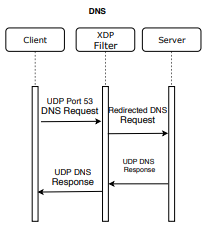
\includegraphics[width=45mm]{./img/dns-process.png}
    \end{center}
    \caption{DNS queries are intercept in XDP and eBPF implementation edits their destination. \cite{rivera2020leveraging}}
    \label{img:dns-process}
  \end{figure}
  XDPにフックされたeBPFプログラムはあるパケットがどのプロセスから送出されるかを認識しており,
  key:プロセス名,value:宛先のハッシュマップを参照してクエリのアドレスを書き換える.
  なお,この研究はDNSクエリを振り分けるキャッシュサーバのリストを指定できるuser-friendlyなインタフェースを提供している.
  
  DoTではTLSで規定された処理を行う必要があるため,AF SocketというXDPの機能を使う.
  先述したように宛先アドレスを編集したあと,AF Socketで作られた仮想ソケットにパケットを送信して
  TCP handshakeやTLSの鍵交換を行う.
  
  DoHにおいては,パケットがカーネルのネットワークスタックに到達する時点でクエリ情報は暗号化されているため,
  平文のDNSやDoTと同様の方法を適用できない.そこでこの研究では,uProbes (user probes) にeBPFプログラムをフックして
  DoHクエリの作成とレスポンスの復号化を監視した.
  uProbesではデータがread-onlyであるためクエリの編集ができないが,その代わりに
  クエリの情報があるキャッシュサーバにどの程度知られているかを計算し,閾値を超えたときにユーザに警告する実装を行った.
  
  \subsubsection{評価}
    Riveraらは\Fref{img:dns-net}に示す実験用ネットワークを構築して提案手法の評価を行った.
    \begin{figure}[tp]
      \begin{center}
        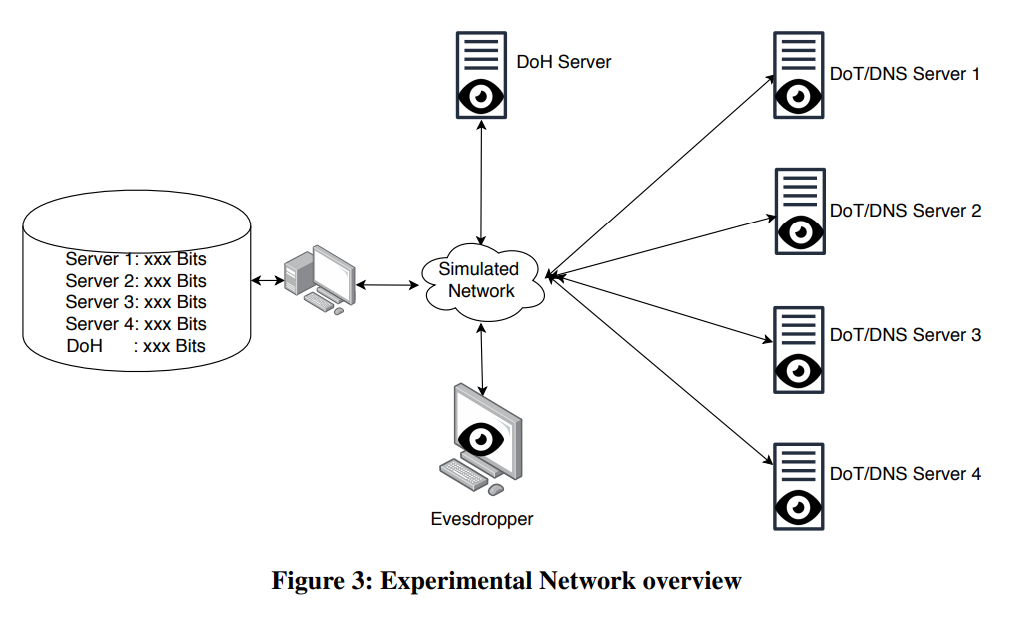
\includegraphics[width=\columnwidth]{./img/dns-eval-net.png}
      \end{center}
      \caption{The overview of the experimental network.}
      \label{img:dns-net}
    \end{figure}
    
    パフォーマンスの評価ではDNSとDoTにおける名前解決時間を計測した.その結果
    DNSでは0.44\%,DoTでは8.15\%のオーバーヘッドが観測された.DoTでのオーバーヘッドが
    大きいのは,AF Socketの処理がボトルネックになっている可能性がある.
    DoHクエリの監視についてはCPUサイクル数を計測し,3.13\%のオーバーヘッドが見られた.
    
    プライバシーの評価では,\Fref{img:dns-net}に示すキャッシュサーバ4台のそれぞれに
    何ビットのクエリ情報が流出しているかを計算し,de-anonymizationが実行可能であるかどうかを
    評価した.
    DoT単体ではISPによるde-anonymizationが実行可能であったが,
    DoTとeBPFを組み合わせた提案手法はクエリを異なるサーバにロードバランスすることで
    de-anonymizationを防ぐことができることが示された.
    
  \subsection{Programmabilityの高いシステムコールフィルタ \cite{jia2023programmable}}
    本研究はLinuxのシステムコールのフィルタリング機構であるseccompの問題点を論じた.
    そしてseccomp-bpfをeBPFに対応させることでフィルタに高いprogrammabilityを与え,
    既存のseccomp-bpfよりも厳密なセキュリティポリシーを適用するためのデザインの提案と実装を行った.
    
    \subsubsection{問題}
      システムコールフィルタとは,システムコールのエントリーポイントにおいてそのシステムコールが
      発行されることを許可または拒否するメカニズムのことを指す.
      seccomp-bpfはプロセスごとに異なるフィルタをcBPFで記述して適用することができ,
      カーネル空間で実行されるためパフォーマンスが優れている.
      
      しかしcBPFがもつ以下の性質により,seccomp-bpfはプロセスごとに静的なallow listを
      適用することしかできない.
      \begin{itemize}
        \item ステートレスである
        \item プログラムサイズの上限が小さい (4096命令)
      \end{itemize}
      このため,本来許可するべきではないシステムコールを許可せざるを得なくなって
      セキュリティが劣化したり,複雑なルールを複数のフィルタのチェインで表現しなければならないことで
      実行効率が低下したりする.
      
      seccomp-bpfの機能を補うためにseccomp notifier \cite{TheSecco46:online} が提案された.notifierは
      システムコールが発行されるたびに実行コンテキストをユーザー空間からカーネル空間に移し,
      そのシステムコールを許可または拒否する判断を行う仕組みである.
      フィルタのprogrammabilityは高いものの,コンテキストスイッチに起因するオーバーヘッドが大きい.
      
    \subsubsection{デザインと実装}
      本研究では既存のseccomp-bpfをseccomp-cBPF,提案手法をseccomp-eBPFと呼び区別している.
      seccomp-cBPFに欠落しているがシステムコールフィルタが有していると望ましい性質として,Jieらは4点を挙げていた.

      1点目はstatefulnessである.statefulなフィルタはシステムコールの発行回数や頻度を記憶して
      フィルタを運用することができる.また,プログラムの実行フェイズに応じて許可するシステムコールの集合を変化させる
      precise temporal specializationも可能になる.
      
      2点目はexpressivenessである.無駄のないフィルタを記述することでフィルタの効率が改善する.
      
      3点目はsynchronizationである.システムコールの競合状態を利用する脆弱性が報告されており,
      そのような脆弱性の原因となるシステムコールが並列に実行される場合に同期を取って競合状態を回避する.

      4点目はsafe user memory accessである.システムコールの引数に
      ポインタ型の変数が渡される場合,そのポインタが指す構造体を検査することはフィルタの意思決定において
      有用である.例えば\texttt{open()}システムコールに渡されるポインタは開こうとしているファイル名の文字列を指している.
      
      Jieらはこれら4つの性質を満たしつつ,
      提案システムへの移行を容易にするためにのseccomp-cBPFが想定する脅威モデルを維持する実装を行った.
      seccomp-eBPFの実装で特筆すべき点は以下の通り.
      \begin{itemize}
        \item \texttt{BPF\_PROG\_TYPE\_SECCOMP}をProgram Typeに追加した.
        \item 既存のヘルパー関数を改修,あるいは新規の関数を追加した.
        \item 上記2点を検証するためにeBPF verifierの検証ロジックを変更した.
      \end{itemize}
      
    \subsubsection{評価}
      seccomp-eBPFの機能の1つであるprecise temporal specializationの性能評価を行った.
      実験では\Fref{img:tmp-spec}に示すようにサーバアプリケーションの実行フェーズを
      初期化フェーズと機能フェーズに分け,それぞれのフェーズでのみ実行されるシステムコールの集合$S_{init}とS_{serv}$を
      seccomp-eBPFのフィルタで許可した.これらのフィルタはプログラムの実行フェーズに応じて動的に適用された.
      \begin{figure}[tp]
        \begin{center}
          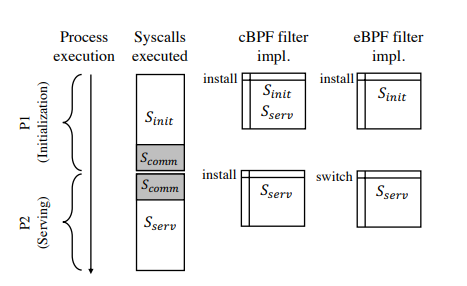
\includegraphics[width=\columnwidth]{./img/tmp-spec.png}
        \end{center}
        \caption{The concept of precise temporal specialization. It should be noted that
        the seccomp-cBPF filter in the initialization phase allows $S_{serv}$.}
        \label{img:tmp-spec}
      \end{figure}
      NGINXやMemcachedといったプログラムを用いて評価したところ,初期化フェーズにおいて33.6\%から55.4\%の
      attack surfaceの削減が見られた.

      さらに,precise temporal specialization以外に追加されたセキュリティ機能も評価された.
      システムコールの実行回数を制限するcount limitingはCVE-2016-0728などの脆弱性をブロックし,
      またserializationの機能はCVE-2018-18281を防ぐことに成功した.
      
      パフォーマンスの評価では,\texttt{getpid()}システムコールを実行するマイクロベンチマークと,
      サーバアプリケーションのベンチマークによるマクロベンチマークを扱った.

      マイクロベンチマークの結果を\Fref{img:micro-bench}に示す.
      \begin{figure}[tp]
        \begin{center}
          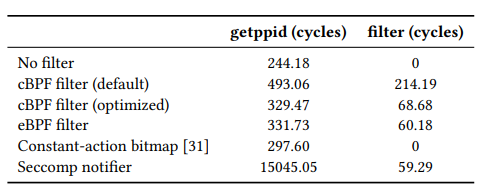
\includegraphics[width=\columnwidth]{./img/micro-bench.png}
        \end{center}
        \caption{Execution time of \texttt{getpid()} with different filters and filter execution time.}
        \label{img:micro-bench}
      \end{figure}
      seccomp-eBPFのフィルタは,seccomp-cBPFのフィルタよりもセキュリティが向上しているにも関わらず,
      コンパイル時最適化を適用したseccomp-cBPFのフィルタと同程度のパフォーマンスを出した.
      notifierのフィルタはシステムコール自体の実行時間を45倍程度大きくし,顕著な性能低下が見られた.

      マクロベンチマークの結果を\Fref{img:macro-bench}に示す.図中の"hybrid"は
      seccomp-cBPFとnotifierを組み合わせたフィルタである.
      \begin{figure}[tp]
        \begin{center}
          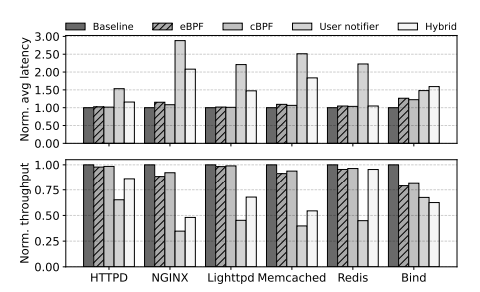
\includegraphics[width=\columnwidth]{./img/macro-bench.png}
        \end{center}
        \caption{Execution time of \texttt{getpid()} with different filters and filter execution time.}
        \label{img:macro-bench}
      \end{figure}
      同じ機能を実装したフィルタを適用した条件で,
      \Fref{img:macro-bench}に示されるサーバアプリケーションを公式のベンチマークを用いて
      レイテンシとスループットを評価した.
      アプリケーションごとに差異は見られるが,マイクロベンチマークの結果と同様の傾向が見られた.
  
  \subsection{周辺機器からLinuxを保護するフレームワーク\cite{tian2019lbm}}
    本研究はBadUSBなどの悪意ある周辺機器を用いた攻撃や,周辺機器のプロトコルスタックのバグを突いた攻撃から
    Linuxを保護するためのフレームワークを提案した.

    \subsubsection{問題}
      本研究が対象としている周辺機器はUSB,Bluetooth,NFCの3種類である.
      周辺機器は各々のプロトコルに則ったパケットをカーネルとやり取りすることで動作するため,
      attack surfaceとして悪意あるパケットを送信する方法と,カーネル側のプロトコルスタックの脆弱性を攻撃する
      方法が考えられる.

      しかしながら,USBを対象とした攻撃には系統的な対策が存在する \cite{tian2016making}が,
      BluetoothやNFCには存在しない.
      したがって,様々な周辺機器に対応することができる包括的なセキュリティフレームワークが必要である.
      
    \subsubsection{デザインと実装}
      この研究では,様々なプロトコルを扱うことができる拡張性の高いフレームワークとしてLBM,Linux (e)BPF Modules
      を提案した.
      そして,サポートする周辺機器のすべての入力と出力を検査すること,新しい周辺機器プロトコルの
      サポートが容易であること,オーバーヘッドの小さいことなどを含むLBMが備えるべき7つの性質を整理した.
      
      TianらはスタンドアローンなコンポーネントとしてLBMを実装した.
      \Fref{img:kernel-design}にカーネル側のシステムの概要を示す.
      \begin{figure}[tp]
        \begin{center}
          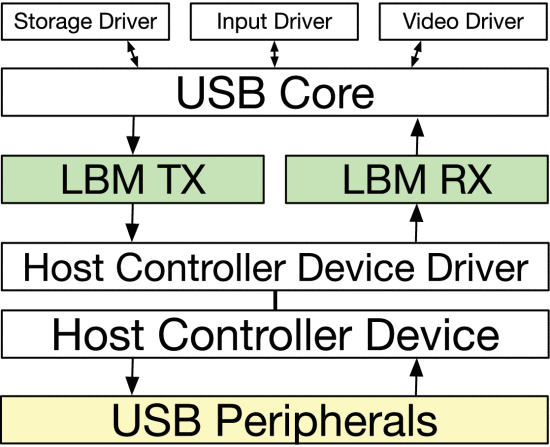
\includegraphics[width=\columnwidth]{./img/sodapdf-converted.png}
        \end{center}
        \caption{The overview of LBM in kernel side. \cite{tian2019lbm}}
        \label{img:kernel-design}
      \end{figure}
      eBPFでフィルタを適用するにあたって,eBPFプログラムのフックに2つのルールを定めている.
      \begin{enumerate}
          \item eBPFプログラムをハードウェアのなるべく近くにフックする (フィルタが回避されることを防ぐため).
          \item 特定のハードウェアの実装に依存しない (拡張性を高めるため).
      \end{enumerate}
      このルールを満たすために,LBM TX (周辺機器への入力)とLBM RX (周辺機器からの出力) のフックポイントは
      プロトコルスタックの下かつLinuxホストのコントローラーデバイスの上に配置された.
      
      LBMを利用するユーザにはLBMTOOLというフロントエンドを提供した.
      ユーザがPCAPに似たドメイン固有言語でフィルタのルールを記述すると,LBMTOOLはそれをコンパイルして
      eBPFプログラムを生成し,フックポイントにロードする.
      
    \subsubsection{評価}
      LBMの評価にあたって,本研究では既知の攻撃を実施するケーススタディとベンチマークによるパフォーマンス計測を行った.

      まずケーススタディでは,レスポンスパケットの先頭2バイトからパケット長をチェックすることで
      スタックを保護するフィルタを記述することができた.
      またUSB充電器を装ったBadUSBを充電は妨害せずにブロックできること,
      Bluetoothの脆弱性の一つであるBlueBorne\cite{BlueBorn43:online}を10行程度のルールで対策できることを示した.
      さらに概念実証としてLBMによるNFCのサポートを行った.その結果カーネルとLBMTOOLへのソースコードの変更は
      合計で100行未満であり,拡張性の高さを表す根拠が得られた.

      ベンチマークによるパフォーマンス計測では,マイクロベンチマークとマクロベンチマークが使用された.
      マイクロベンチマークはRXパスで10,000のパケットをカウントし,LBMがもたらすオーバーヘッドを計測した.
      その結果を\Fref{img:usb-latency}に示す.\Fref{img:usb-latency}によると,JITコンパイル
      最適化が行われた場合LBMのオーバーヘッドは,パケットあたり1$\mu s$程度であった.
      \begin{figure}[tp]
        \begin{center}
          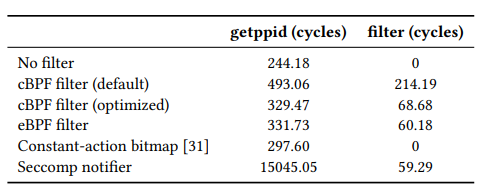
\includegraphics[width=\columnwidth]{./img/micro-bench.png}
        \end{center}
        \caption{LBM overhead in $\mu s$ measured on 10K packets on the RX path. 
        For each subsystem, the 1st row is for normal LBM and the 2nd row is for LBM-JIT.\cite{tian2019lbm}}
        \label{img:usb-latency}
      \end{figure}

      マクロベンチマークでは,filebenchというベンチマークを採用してUSB3.0外部ストレージへのファイル書き込みのスループットを計測した.
      その結果を\Fref{img:file-bench}に示す.VanillaはLBMが組み込まれていない純正のLinuxカーネルを意味している.
      \begin{figure}[tp]
        \begin{center}
          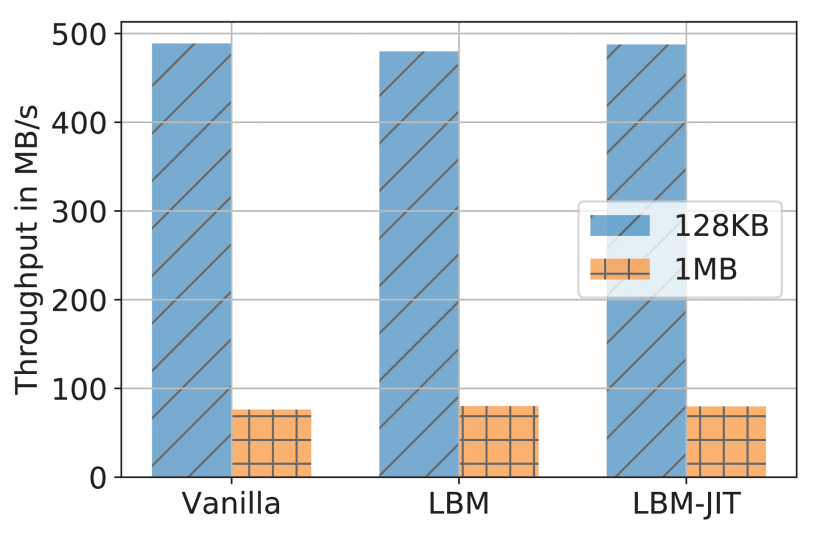
\includegraphics[width=\columnwidth]{./img/macro-graph.png}
        \end{center}
        \caption{Throughput of USB 3.0 external storage with filebench. \cite{tian2019lbm}}
        \label{img:file-bench}
      \end{figure}
      いずれの条件でも同様のスループットが得られており,LBMのオーバーヘッドが小さく抑えられていることを示している.
      なお,平均ファイルサイズが大きくなるとスループットが極端に落ちる現象はページキャッシュサイズに由来する.
      
      さらにBluetoothに対しても\texttt{l2ping}によるRTTの計測が行われた.\Fref{img:file-bench}の3種類の設定でRTTを計測したところ
      いずれも5$ms$付近の結果が得られた.LBMによる1パケットあたりの遅延は1$\mu s$であったから,RTTと比較すると遅延は無視できる範囲に収まった.
      % cloud nativeの話で0.5ページ, cloudflareで1ページ弱,abstractと「はじめに」で0.5ページ

\section{おわりに}
  本稿では,eBPFという技術の発展の歴史,アーキテクチャ,主要なユースケースについて述べた後,
  eBPFを活用したセキュリティシステムを提案する既存研究の取り組みを紹介した.
  eBPFが提供するシステムの可観測性,セキュリティ,高パフォーマンスはセキュリティ技術者および研究者にとって
  強力な武器であり,これまで以上に多岐にわたる問題に対処できるようになったことがわかる.

  eBPFは比較的新しい技術であり,既に広く普及していながらも未だ発展途上である.
  今後もクラウドネイティブ環境を中心に新規のユースケースが提案されることが期待される.

\bibliographystyle{unsrt}
{
\footnotesize
\bibliography{bib}
}

\end{document}
